\newpage




\section{Pointer Analysis}

Pointer analysis is a compile-time technique that helps identify relationships between pointer variables and the memory locations that 
they point to during program execution. Pointers are powerful programming constructs and allow complex memory manipulation during program 
execution through techniques such as pointer arithmetic and dynamic memory allocation. Pointer relationships can thus be complex and difficult 
to analyze at compile time. On the other hand, however, they provide the benefit of simplifying various other compile time analyses such as 
constant propagation, alias analysis in C programs that allow extensive use of pointers.\cite{Pointsto7:online}



Potential applications of pointer analysis for multithreaded programs include:
the development of sophisticated software engineering tools such as race detectors, memory leak detectors, wild pointer detectors and program slicers; 
memory system optimizations such as prefetching
and moving computation to remote data; automatic batching of long latency
file system operations; support parallelism in different levels: instruction-level parallelism and thread-level parallelism ;
and to provide information required to apply traditional
compiler optimizations such as constant propagation, common subexpression
elimination, register allocation, code motion and induction variable elimination
to multithreaded programs.\cite{rugina2003pointer}

\begin{definition}{Aliases}
    Two variables are aliases if they reference the same memory location.
\end{definition}


\begin{definition}{The	Pointer	Alias	Analysis	Problem	}
    Decide for every pair of pointers at every program point: do they point to the same memory location?
\end{definition}

\subsection{Background}

A pointer alias analysis attempts to determine when two pointer expressions refer to the same storage location. A
points-to analysis , or similarly, an analysis based
on a compact representation , attempts to determine what storage locations a pointer can point to. This
information can then be used to determine the aliases in the program. Alias information is central to determining what
memory locations are modifed or referenced.

There are several dimensions that aect the cost/precision
trade-offs of interprocedural pointer analyses. How a pointer
analysis addresses each of these dimensions helps to categorized the analysis. An empirical comparison with a 
difference in more than one dimension can limit the usefulness of
the comparison. Some of the dimensions are

\textbf{ Flow-sensitivity:} Is control-ow information of a procedure used during the analysis? By not considering control
ow information, and therefore computing a conservative
summary, ow-insensitive analyses compute one solution for
either the whole program or for each method, whereas a ow-sensitive analysis computes a solution for each program point. 
Flow-insensitive analyses thus can be more efficient, but less precise than a ow-sensitive analysis. Flow-insensitive analyses
are either equality-based, which treat assignments as bidirectional and typically use a union-find data structure, 
or subset-based, which treat an assignment as
a unidirectional ow of values.

\textbf{ Context-sensitivity:} Is calling context considered when
analyzing a function or can values ow from one call through
the function and return to another caller?

\textbf{ Heap modeling:} Are ob jects named by allocation site,
or is a more sophisticated shape analysis performed?

\textbf{ Aggregate modeling:} Are elements of aggregates distinguished or collapsed into one object?

\textbf{ Whole program:} Does an analysis require the whole
program or can a sound solution be obtained by analyzing
only components of a program?

\textbf{ Alias representation:} Is an explicit alias representation [51, 64] or a points-to/compact representation used?


\subsection{Flow-Sensitivity}

Flow-sensitive pointer analysis respects a program’s control flow
and computes a separate solution for each program point, in contrast to a flow-insensitive analysis, 
which ignores statement ordering and computes a single solution that is conservatively correct for
all program points.


\begin{figure}[H]
	\centering
	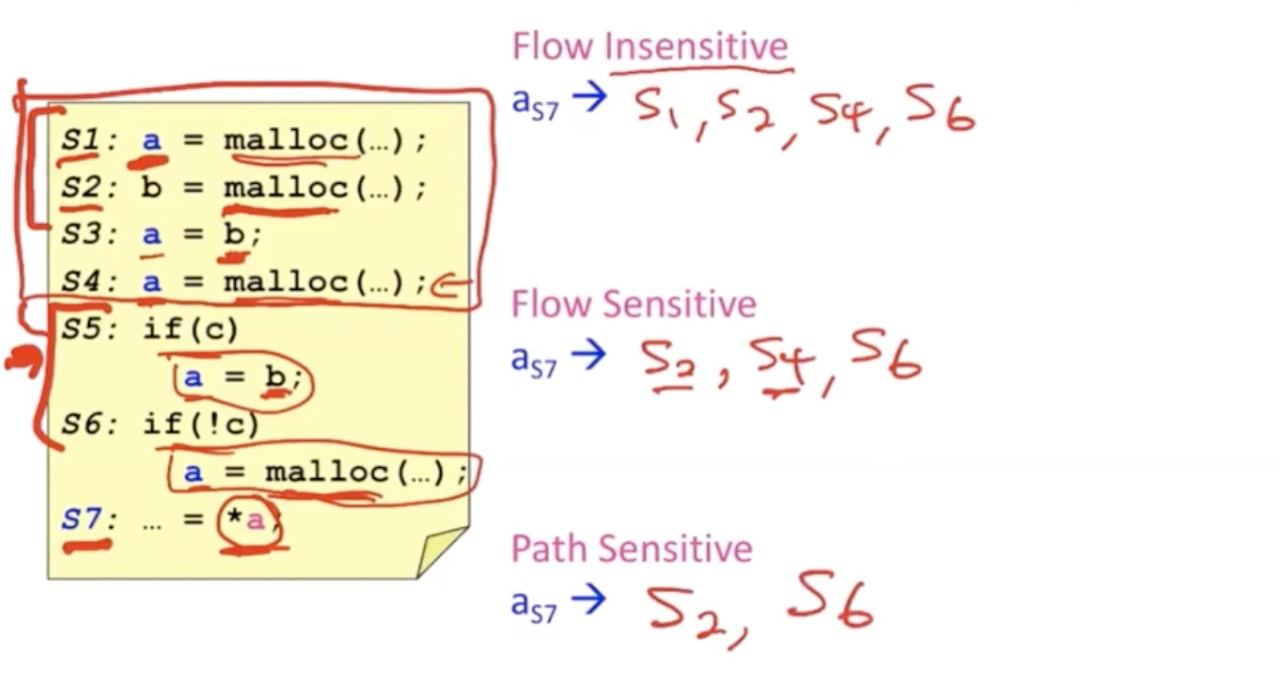
\includegraphics[width=0.7\textwidth]{p127.jpg}
	\caption{Flow-sensitive vs. flow-insensitive analysis}
	\label{fig:p127}
\end{figure}


\subsection{Context-sensitive }


Context sensitivity has a most significant impact on analysis precision due to separate
treatment for each method in the program. In practice, each time analysis considers new
method call it creates a new structure that represents unique method scope in the memory.
It treats all read/write operations inside this method in scope of this context and makes this
information available later for its processing.


\begin{figure}[H]
	\centering
	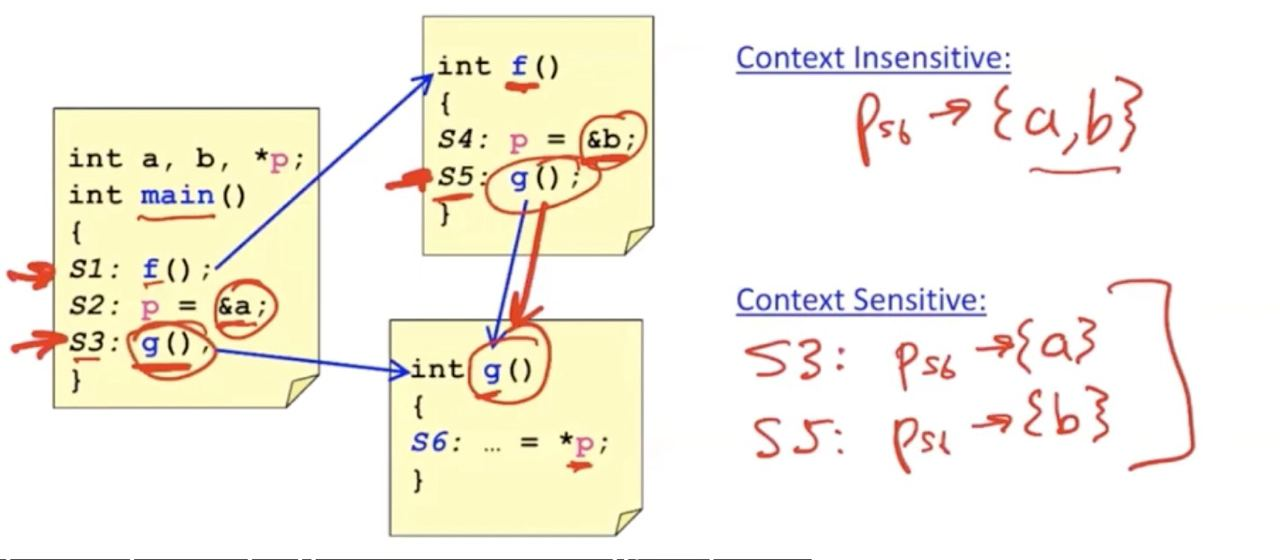
\includegraphics[width=0.7\textwidth]{p128.jpg}
	\caption{Context-sensitive vs. Context-insensitive analysis}
	\label{fig:p128}
\end{figure}



\subsection{Modeling Aggregates}
A key implementation detail is whether aggregate com-
ponents are distinguished or summarized into one object.
C/C++'s weak typing makes this diÆcult to address cor-
rectly. Thus, most published work does not distinguish ag-
gregates. However, this diÆculty does not exist in a strongly-
type language like Java, and therefore, components should
be distinguished in such languages. Most recent work
has chosen to distinguish components. Unfortunately, few researchers have studied the impact of this decision.